\chapter{Simulation}

As P--ONE has only deployed the Pathfinder missions thus far, including STRAW and STRAWb, the data used in this thesis is primarily simulated. In particular, the data needs to be usable to test and build a reconstruction algorthim for muon--neutrinos. This means simulating muon tracks. The following section covers the simulation process used to produce the data including the pre--existing IceCube Framework, simulating neutrinos, simulating muons and the detector response. 

\section{IceCube Framework}

The software framework already exists from IceCube, and in order to minimize the amount of new code needed to simulate P--ONE it is simplest to use the IceCube software. In particular, the software documentation is readily available \cite{icetray, icetray_art} and referred to as IceTray. This is meant to be a full framework capable of simulating, reconstructing and analyzing all in one \cite{icetray, icetray_art}. For the purposes of P--ONE, only the simulation subset of the framework is used as it is primarily made using open--source software, and hence can avoid potential proprietary issues.

The bulk of the code is written in C++ with the goal of being modular. This means that rather than writing scripts that call functions or classes that are pre--existing, the code is designed so that there is a single steering script that calls modules to run tasks including the simulation of muons or neutrinos, and including geometry files. Modules can be added by users as well to then be included in the steering scripts. The code has also been wrapped using Python so that modules can be reached via python scripts, and hence steering scripts can be written in Python. For this reason, Python is the language of choice for the purposes of this work.

Due to the nature of data collected by neutrino telescopes, the Icetray framework was developed to handle working with photon tables in a manageable manner. Photon propogation and simulation at reconstruction time is an intensive process, and for real events is avoided by using simulations done apriori to construct tables that can be used at event analysis time \cite{icetray_art}. The tables generated must be massive for this reason, and the Icetray framework works around this issue by allowing each module to work independently of the others with output queues so that the underlying topology of the modules is generally non-linear and can be quite complex. As the data needed to be simulated for this work, the photons were simulated as well, though tables may be used in the future. A more detailed explaination of Icetray can be found here \cite{icetray_art}.

\section{Simulating Neutrinos}

The Icetray sofware used to generate neutrinos is the very aptly named Neutrino--Generator (NuGen) \cite{icetray, icetray_art}. This is code written in IceTray based off of the All Neutrino Interaction Generator (ANIS), a high energy neutrino generator used for neutrino telescopes developed originally for AMANDA \cite{lepton_inj}. NuGen uses a cylinder in which the events are generated to inject the neutrinos into the detection volume \cite{sim_present}. The main purpose of the cylinder is to provide the user with control over where the neutrinos are generated without exact positions. As a neutrino telescope primarily aims to detect neutrinos that have traveled through the earth, NuGen uses an Earth model to measure the density to use when computing the interaction probability. As described in \cite{sim_present}, NuGen computes the track length inside the earth and inside the detection volume seperately and then computes step--wise the path of the neutrino checking each step if it interacts with the earth using the depth and cross--section. If ever an interaction occurs, it will decide the interaction randomly and produces secondaries. These are then propogated until they reach the detector volume. A propogation probability and interaction probability are computed of the interaction, and then the neutrino is weighted for use when predicting fluxes. This weight is defined as
\begin{equation}
  w_{i} = \frac{OneWeight_{i}}{NEvents}\times \frac{d\Phi_{\nu}(E_{\nu})}{dE_{\nu}} \, ,
\end{equation}
where
\begin{equation}\label{eq:one_weight}
  OneWeight = \left(\frac{P_{\text{int}}}{E^{-\gamma}}\right)\cdot \int_{E_{\text{min}}}^{E_{\text{max}}}E^{-\gamma}dE\cdot Area\cdot \Omega \cdot T[\text{Gev}\cdot cm^{2}\cdot s\cdot sr]
\end{equation}.
In Equation \ref{eq:one_weight}, $P_{\text{int}}$ is the total interaction probability weight, $E^{-\gamma}$ is the neutrino generation energy spectrum shape, $E_{\text{min}}$ and $E_{\text{max}}$ is the minimum and maximum generation energy of neutrinos, $Area$ is the generation area, $\Omega$ is the solid angle and $T$ is 1 second and the timescale.

The lepton propogation is carried out by PROPOSAL, more software used by IceCube. PROPOSAL accounts for stochastic energy losses due to ionization, positron-electron pair production, bremsstrahlung, photo-nuclear interactions and decay \cite{sim_present}. The photon propogation is handled by CLSim, which accounts for optical properties of the medium and absorption/scattering interactions. This can be done in either a parallel or series manner by using either GPUs or CPUs respectively. 

\section{Simulating Muons}

The module used to generate muons is the MuonGun that exists in GEANT4. This can be used to inject muons based on some sampling surface dependent upon a given flux model \cite{icetray}. Muon Gun is versatile as it can be easily modified to produce muons using a variety of sampling surfaces, and can even be modified to be energy dependent \cite{icetray}. Muon Gun works by drawing samples from a parameterization/fit of the atmospheric muon flux \cite{icetray,muon_param}, and for this work the flux model used is the one created by IceCube \cite{icetray} where fits are made to CORSIKA \cite{corsika} simulations with SIBYLL \cite{sibyll} wieghted to the spectrum by Hoerandel \cite{hoerandel}. Understanding this requires understanding the muon background source.

\subsection{Cosmic Ray Muons}

As discussed in Section \ref{subsec:atmos}, neutrinos can be produced in the atmosphere from cosmic ray interactions. Another byproduct of these interaction cascades are muons \cite{corsika, sibyll}, which can become a background in neutrino telescopes and require characterization. To understand this background source at the detector level, the muon flux needs to be tracked back to the source of the atmosphere and the cosmic ray flux. The cosmic ray flux used to develop the parameterized forms found in \cite{muon_flux} and the fits in \cite{icecube} is based off of the specturm described by Hoerandel in \cite{hoerandel}.

Predicting the cosmic ray flux is no walk in the park. Ignoring theoretical models to predict the sources and build a model that way, which is still covered in \cite{hoerandel} but of no real consequence for the purposes of this text, Hoerandel introduces the \textit{poly--gonato} model. This is the method used to fit the observed energy distribution of cosmic rays for different types of cosmic rays. These range from protons to heavier nuclei like iron \cite{hoerandel}. This can accurately describe the observed energy spectrum and mass composition in the energy range from 10 GeV to atleast 100 PeV. In particular, this model accurately describes the first ``knee'' at 4.5 PeV in the energy spectrum with subsequent cut-offs for individual elements, starting with protons, and the second ``knee'' at 400 PeV with the end of the galactic component \cite{hoerandel}. 

With the cosmic ray flux modeled, the interactions to produce the showers with the muons in them still need to be simulated. The softwares used to do these simulations are Cosmic Ray Simulations for KASCADE (CORSIKA) and Sibyll (atmospheric cascade event generator). CORSIKA is a Monte Carlo program for studying air showers produced by cosmic rays (photons, protons, nuclei, and any other high energy particle) \cite{corsika}. CORSIKA, though originally developed for the KArlsruhe Shower Core and Array DEtector (KASCADE) \cite{kascade} a detector built for examining high energy cosmic rays, has now developed and evolved into a versatile tool used in energy ranges from $10^{12}$ eV to energies above $10^{20}$ eV. In order to maintain accuracy, CORISKA is detailed in tracking and recording the path and processes of every secondary produced. Due to lack of experimental data in extreme energy regimes, Sibyll is used as an event generator to circumvent this issue. 

\subsection{Flux Model}

Now that the production step is understood in the simulation, the only thing that remains is the muon flux and spectrum at the detector level. The energy parameterization is well described in \cite{muon_flux}; it depends on the water depth ($h$), zenith angle ($\theta$), multiplicity, and energy. In particular, the energy spectrum of single muons is described by
\begin{equation}
  \frac{dN}{d(\log_{10}E_{\mu})} = G\cdot E_{\mu}e^{\beta X(1 - \gamma)}\left[E_{\mu} + \epsilon(1 - e^{-\beta X})\right]^{-\gamma}\, ,
\end{equation}
where $\epsilon$, $\gamma$, and $\beta$ are simple fit parameters, $X=h/\cos\theta$, and $G$ is a normalization factor \cite{muon_flux}. The flux can similarly be paramterized and fit to data. Unfortunately, this was found to be unsatisfactory for icecube \cite{icetray}, as the fitting ended up being more sensitive than expected and ultimately yielded unsatisfactory results.

Generating muons by beginning at the cosmic ray level is inherently a slow process, as not all produced secondaries are muons, and they may not even hit the detector. This becomes a massive computational load, and hence another method was used by IceCube to simulate the muons. To force an interaction at the muon level, the physics and behaviours of the cosmic ray interaction down to the muon hitting the detector are simulated, tabulated and fit using tensor--product B--splines from the Photospline package to fit between bins \cite{icetray}. These tables now can be referenced at the muon production step for both the energy and flux, where the latter is defined by giving the muon a weight.

It is important here to understand here that these steps included the medium in which the detector sits, which is ice for IceCube. This means when considering any form of analysis on rates, the flux model must be examined a bit closer than just assuming it works for P--ONE aswell. For the purposes of testing reconstruction capabilities, however, this is more than enough and the tables having been built with ice in mind is a non-issue. 

The energy loss due to water interactions also have to be added and are also discussed in \cite{muon_flux}. These fits are great for fast generation of muons \cite{muon_flux, icetray}, which is important for understanding the background of cosmic ray muons common in most neutrino telescopes \cite{icecube, antares, amanda, pone, muon_flux}. In particular, all of the simulated data referenced in Chapter \ref{ch:results} is made using a particular version of Muon Gun referred to as 'GenerateCosmicRayMuons', which is just a module that calls Muon Gun with presets for a particular direction of Muons (down heading through the detector).

\section{Detector Response}

Another aspect that has to be simulated is the response of the detector. This involves producing pulses from propogated photons that hit particular PMTs. This step can then include noise, efficiency, and directionality of the PMT. The noise would account for the dark noise that is present in standard PMTs \cite{ham}, but also the noise that arises from other potential background sources. The efficiency of the PMT also can reduce the statistics \cite{ham}. The directionality provides information on whether or not the photon that reaches the detector actually hits the detection side of the PMT, as otherwise it could be reflected or absorbed. Of these detector responses, the directionality is the only one implemented for this data. The noise and efficiency introduce complexity to the system that has been ignored for the purposes of testing the reconstruction in a controlled environment before introducing noise/efficiency and folding that into the likelihood space. Another aspect to consider is the distribution of the DOMs in space: the geometry.

The choice of geometry is incredibly important, as varying the position and number of detectors can, as one would expect, result in large changes in the performance of the detector. The current proposed first stage of P--ONE is to be a pair of nested circles with the inner containing three strings and the outer containing 7 \cite{pone}, as we can see in Figure \ref{fig:pone_geo}. The simulated geometry is based off of this first design and held in a ``.gcd'' file which is used by IceTray \cite{icetray} and is plotted in Figure \ref{fig:pone_3d}. If we wish to see how the potential detector performance is affected by varying the geometry, we can change this geometry file and measure parameters such as the effective area to see how well it compares.

\begin{figure}[H]
  \centering
  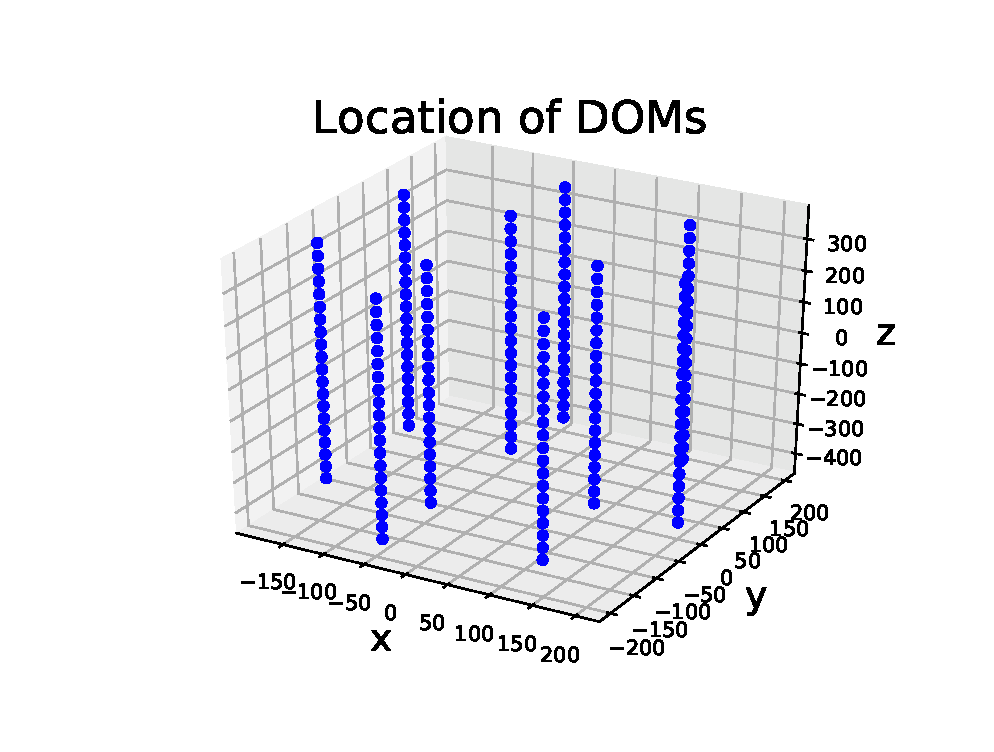
\includegraphics[width=12cm]{./Figures/reco_plots/DOM_Locations_3d.eps}
  \caption{The geometry of the current string model used in the simulation and reconstruction efforts. There are a total of 200 DOMs. The relative rotations between the two concentric circles of 3 and 7 strings respectively is zero and has hence not been modified from the default.}
  \label{fig:pone_3d}
\end{figure}

One of the most useful and widely used methods of measuring a neutrino detectors performance at a glance is the effective area. For a given particle of interest with some flux, the effective area is defined as the area of the detector scaled by the efficiency of the detector in measuring this particle \cite{2010icecube}. Another way of phrasing this is that the effective area is that which detects perfectly the particles entering it for a given number of detections. Computing the effective area is non-trivial, as it is particle, flavour, energy, and direction dependent. 
